\tikzstyle{arrow} = [thick,->,>=stealth]

\tikzstyle{program} = [rectangle, minimum width=2.8cm, minimum height=1cm, text centered, node contents=Program, draw=black]

\tikzstyle{abstraction} = [rectangle, minimum width=2.8cm, minimum height=1cm, text centered, node contents=Abstraction, draw=black]

\tikzstyle{apply} = [rectangle, minimum width=2.8cm, minimum height=1cm, text centered, node contents=Apply, draw=black]

\tikzstyle{left} = [rectangle, minimum width=2.8cm, minimum height=1cm, text centered, node contents=Left, draw=black]

\tikzstyle{right} = [rectangle, minimum width=2.8cm, minimum height=1cm, text centered, node contents=Right, draw=black]

\tikzstyle{copy} = [rectangle, minimum width=2.8cm, minimum height=1cm, text centered, node contents=Copy, draw=black]

\tikzstyle{drop} = [rectangle, minimum width=2.8cm, minimum height=1cm, text centered, node contents=Drop, draw=black]

\begin{figure}[htb]
    \centering
    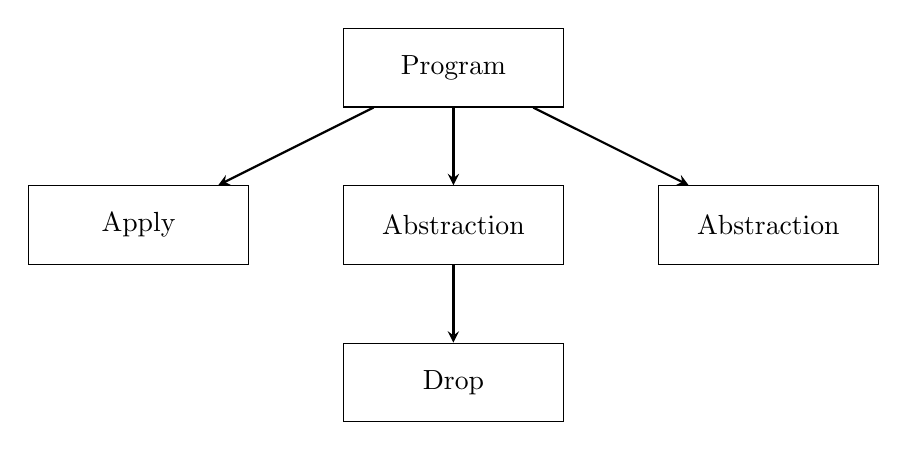
\begin{tikzpicture}[node distance=2cm]
        \node (program) [program];
        \node (2) [abstraction, below of=program];
        \node (1) [apply, left of=2, xshift=-2cm];
        \node (3) [abstraction, right of=2, xshift=2cm];
        \node (4) [drop, below of=2];

        \draw [arrow] (program) -- (1);
        \draw [arrow] (program) -- (2);
        \draw [arrow] (program) -- (3);
        \draw [arrow] (2) -- (4);
    \end{tikzpicture}
    \caption{Kihi intermediary representation of a simple program: \lstinline{apply (drop) ()}}
    \label{fig:kihi_intermediary_representation_example_1}
\end{figure}


% · → × → (· · ← (→ → (·) ×)) (· ← (· · ← ← ()) × → (· · ← (·) · ← ← () · ← (×)) · ← ← ()) (↓)